\sep
\section{Das Riemann Integral}
\subsection{Integrabilitätskriterien}
\Def[5.1] Eine \textbf{Partition} von I ist eine endliche Teilmenge \(P \subsetneq[a, b]\) wobei \(\{a,b\} \subseteq P\)
Eine Partition \(P'\) ist eine Verfeinerung von P falls \( P \subseteq P'\). Offensichtlich ist die Vereinigung \( P_1 \cup P_2\) zweier Partitionen wieder eine Partition, insbesondere haben zwei Partitionen immer eine gemeinsame Verfeinerung.
Sei nun \( f:[a,b] \rightarrow \R\) eine beschränkte Funktion(Def3.1(3)), das heisst es gibt \( M \geq 0\) mit \( \abs{f(x)} \leq M \ \forall x \in [a,b]\). Sei auch \( P= \{x_0, x_1, \dots, x_n\}\) eine Partition von I. Insbesondere gilt:
\[ x_0 = a < a_1 < \dots < x_n =b\]
Wir bezeichnen mit \( \delta_i := x_i - x_{i-1}, \ i \geq 1\), die Länge des Teilintervalls \([x_{i-1,x_i}] \)
Wir definieren die Untersumme
\[s(f,P) := \sum_{i=1}^n f_i \delta_i, \quad f_i = \inf_{x_{i-1} \leq x \leq x_i} f(x)\]
und die Obersumme
\[S(f,P) := \sum_{i=1}^n F_i \delta_i, \quad F_i = \sup_{x_{i-1} \leq x \leq x_i} f(x)\]
Bemerke, dass
\[ -M \leq f_i \leq F_i \leq M\]
somit sind \(s(f,P)\) und \(S(f,P)\) wohldefiniert und es gilt:
\[ -M(b-a) \leq s(f,P) \leq S(f,P) \leq M(b-a)\]
\Lemma[5.2]
\begin{enumerate}
    \item [1] Sei \(P^{'}\) eine Verfeinerung von P, dann gilt:
    \[s(f.P) \leq s(f,P^{'}) \leq S(f, P^{'}) \leq S(f,P)\]
    \item [2] Für beliebige Partitionen \(P_1, P_2\) gilt:
    \[s(f,P_1) \leq S(f, P_2)\]
\end{enumerate}
\Def[5.3] Eine beschränkte Funktion \(f: [a,b] \rightarrow \R \) ist \textbf{Riemann integrierbar} falls
\[s(f) = S(f)\]
In diesem Fall bezeichnen wir den gemeinsamen Wert von \(s(f)\) und \(S(f)\) mit
\[ \int_{a}^{b} f(x) \,dx \]
\Satz[5.4] Eine beschränkte Funtkion ist genau dann integrierbar, falls
\[ \forall \epsilon > 0 \quad \exists P \in \mathcal{P}(I) \ \text{mit} \ S(f,P) - s(f,P) < \epsilon \] 
\Satz[5.8](Du Bois-Reymond 1875)
Eine beschränkte Funktion \(f : [a,b] \rightarrow \R \) ist genau dann integrierbar, falls \( \forall \epsilon > 0 \quad \exists \delta > 0\) so dass
\[ \forall P \in P_{\delta}(I), S(f, P) - s(f, P ) < \epsilon \]
Hier bezeichnet \( P_\delta (I)\) die Menge der Partitionen P für welche \( \max_{1 \leq i \leq n} \delta_i \leq \delta\) \newline
\Korollar[5.9] Die beschränkte Funktion \(f: [a,b] \rightarrow \R \) ist genau dann integrierbar mit \(A:= \int_{a}^{b} f(x) \,dx\) falls:
\( \forall \epsilon > 0 \quad \exists \delta > 0 \) so dass \( \forall P \in p(I) \) Partition mit \( \delta(P) < \delta \) und \( \epsilon_1, \dots, \epsilon_n\) mit
\(\mathcal{E}_i \in [x_{i-1}, x_i], P= \{x_0, \dots, x_n\}\)
\[\abs{ A - \sum_{i=1}^n f(\mathcal{E_i}) ( x_i - x_{i-1}) } < \epsilon \]
\sep
\subsection{Integrierbare Funktionen}
Bis jetzt haben wir gesehen, dass konstante Funktionen sowie die Funktion \( f(x) = x\) auf jedem kompakten Intervall integrierbar sind. \newline
\Satz[5.10] Seien \(f,g : [a,b] \rightarrow \R \) beschränkt, integrierbar und \( \lambda \in \R \). Dann sind \(f+g, \lambda \cdot f, f \cdot g, \abs{f}, \max(f,g), \min(f,g) \) und \( \frac{f}{g}\) ( falls \( \abs{g(x)} \geq \beta > 0 \quad \forall x \in [a,b]\)) integrierbar \newline
\Bem{5.11} Sei \( \phi : [c,d] \rightarrow \R \) eine beschränkte Funktion. Dann ist
\[\sup_{x,y \in [c,d]} \abs{\phi(x) - \phi(y )} = \sup_{ x \in [c,d]} \phi(x) - \inf_{ x \in [c,d]} \phi(x)\]
\Korollar[5.12] Seien P,Q Polynome und \([a,b]\) ein Intervall in dem Q keine Nullstelle besitzt. Dann ist
\[ [a,b] \rightarrow \R \]
\[ x \rightarrow \frac{P(x)}{Q(x)}\]
integrierbar \newline
\Def[5.13] Eine Funktion \(f: D \rightarrow \R, \quad D \subseteq \R  \) ist in D \textbf{gleichmässig stetig}, falls
 \[ \forall \epsilon > 0 \quad \exists \delta > 0 \quad \forall x,y \in D : \]
\[ \abs{x-y} < \delta \implies \abs{f(x) - f(y)} < \epsilon \]
\Bsp[5.14] Die Funktion \( f: \R \rightarrow \R, \  x \rightarrow x^2\) ist auf \( \R \) stetig aber nicht gleichmässig stetig. \newline
\Satz[5.15] (Heine 1872). Sei \(f : [a,b] \rightarrow \R\) stetig in dem kompakten Intervall \([a,b]\). Dann ist f in \([a,b]\) gleichmässig stetig. \newline
\Satz[5.16] Sei \(f: [a,b] \rightarrow \R \) stetig. Dann ist f integrierbar \newline
\Satz[5.17] Sei \(f: [a,b] \rightarrow \R\) monoton. Dann ist f integrierbar \newline
\Bem[5.18] Seien \(a < b < c \) und \(f : [a.c] \rightarrow \R \) beschränkt mit \(f |_{[a,b]}\) und \(f |_{[b,c]}\) integrierbar. Dann ist f integrierbar und
\[ \int_{a}^{c} f(x) \,dx = \int_{a}^{c} f(x) \,dx + \int_{b}^{c} f(x) \,dx \]
\Def{} Wir erweitern unsere Definiton von Integralen
\[ \int_a^a f(x) dx = 0  \ \text{und falls} \ a < b\]
\[ \int_b^a f(x) dx := - \int_a^b f(x) dx\]
\Satz[5.19] Sei \(I \subsetneq \R \) ein kompaktes Intervall mit Endpunkten a,b sowie \(f_1, f_2 : I \rightarrow \R \)  beschränkt integrierbar und \( \lambda_1, \lambda_2 \in \R \). Dann gilt:
\[ \int_{a}^{b} ( \lambda_1 f_1(x) + \lambda_2 f_2(x)) \,dx = \]
\[\lambda_1 \int_{a}^{b} f_1(x) \,dx + \lambda_2 \int_{a}^{b} f_2(x) \,dx \]
\sep
\subsection{Ungleichungen und Mittelwertsatz}
Nebst Linearität(S5.19) hat das Riemann Integral auch eine Monotonieeigenschaft; diese wiederum führt zum Mittelwertsatz der die basis des Fundamentalsatzes der Differentialrechnung bildet.
\Satz[5.20] Seien \(f,g : [a,b] \rightarrow \R \) beschränkt integrierbar, und
\[ f(x) \leq g(x) \quad \forall x \in [a,b]\]
Dann folgt:
\[ \int_{a}^{b} f(x) \,dx \leq \int_{a}^{b} g(x) \,dx \]
\Korollar[5.21] Falls \(f: [a,b] \rightarrow \R \) beschränkt integrierbar, folgt
\[ \abs{ \int_{a}^{b} f(x) \,dx} \leq \int_{a}^{b} \abs{f(x)} \,dx \]
\Satz[5.22](Cauchy-Schwarz Ungleichung 1821)
Seien \(f,g : [a,b] \rightarrow \R \) beschränkt integrierbar. Dann gilt:
\[ \abs{\int_{a}^{b} f(x) g(x) \,dx} \leq \sqrt{\int_{a}^{b} f^2(x) \,dx} \sqrt{\int_{a}^{b} g^2(x) \,dx }\]
\Satz[5.23](Mittelwertsatz, Cauchy 1821) \newline
Sei \(f: [a,b] \rightarrow \R \) stetig. Dann gibt es \(\mathcal{E} \in [a,b]\) mit:
\[ \int_{a}^{b} f(x) \,dx = f(\mathcal{E})(b-a)\]
\Bsp[5.24] Die Stetigkeit ist eine wichtige Vouraussetzung:
Sei
\begin{equation}
f:[0,1] \longrightarrow \mathbb{R}, \quad f(x)= \begin{cases}0 & 0 \leq x<\frac{1}{2} \\ 1 & \frac{1}{2} \leq x \leq 1\end{cases}
\end{equation}
Dann ist
\[ \int_0^1 f(x) \,dx = \int_0^{\frac{1}{2}} 0 \,dx + \int_{\frac{1}{2}}^1 1 \,dx = \frac{1}{2}\]
\Satz[5.25](Cauchy 1821) Seien \(f,g : [a,b] \rightarrow \R \) wobei f stetig, g beschränkt integrierbar mit \(g(x) \geq 0 \quad \forall x \in [a,b]\). Dann gibt es \(\mathcal{E} \in [a,b] \) mit
\[ \int_{a}^{b} f(x)g(x) \,dx = f(\mathcal{E}) \int_{a}^{b} g(x) \,dx \]
\sep
\subsection{Fundamentalsatz}
Dieser Satz, auch Fundamentalsatz der Analysis genannt, besagt, dass die Ableitung die Umkehrung des Integrals ist. Dieser Satz hat vielseitige Anwendungen, unter anderem die Berechnung von Flächeninhalten und Längen von Kurven \newline
\Satz[5.26] Seien \(a < b\) und \(f: [a,b] \rightarrow \R \) stetig. Die Funktion
\[F(x) = \int_{a}^{x} f(t) \,dt \quad a \leq x \leq b\]
ist in \([a,b]\) stetig differenzierbar und
\[ F'(x) = f(x) \quad \forall x \in [a,b]\]
\Def[5.27] Sei \( a < b\) und \(f: [a,b] \rightarrow \R\) stetig. Eine Funktion \(F: [a,b] \rightarrow \R\) heisst \textbf{Stammfunktion} von f, falls F (stetig) differenzierbar in \([a,b]\) ist und \(F'=f\) in \([a,b]\) gilt \newline
\Satz[5.28] (Fundamentalsatz der Differentialrechnung) Sei \(f:[a.b] \rightarrow \R \) stetig. Dann gibt es eine Stammfunktion F von f, die bis auf eine additive Konstante eindeutig bestimmt ist und es gilt: 
\[ \int_{a}^{b} f(x) \,dx = F(b) - F(a)\]
\Bsp[5.29]
\begin{enumerate}
    \item \(f(x) = x\)
    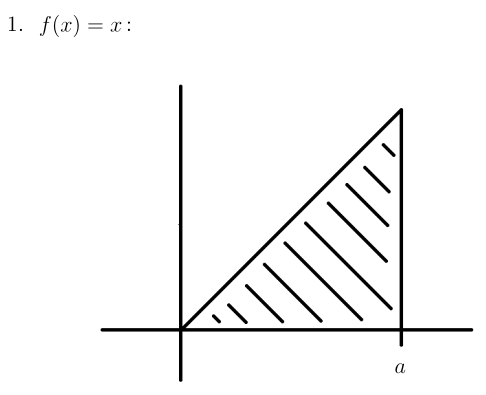
\includegraphics[scale=0.255]{Stammfunktion1.png}
    Dann ist \( \frac{x^2}{2}\) eine Stammfunktion von f und folglich:
    \[ \int_0^a x \,dx = \frac{a^2}{2} \]
    \item \(f(x) = x^2 \)
    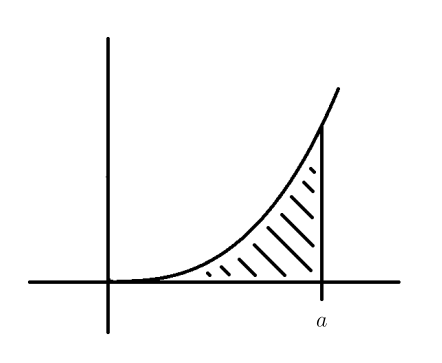
\includegraphics[scale=0.255]{Stammfunktion2.png}
    Dann ist \( \frac{x^3}{3}\) Stammfunktion von f und folglich
    \[ \int_{0}^{a} x^2 \,dx = \frac{a^3}{3}\]
\end{enumerate}
Zur Berechnung von Integralen und Stammfunktionen werden wir zwei Rechenregeln aus dem Fundamentalsatz herleiten. Es handelt sich um Partielle Integration und Substitution. \newline
\Satz[5.30](Partielle Integration) Seien \(a < b\) reele Zahlen und \(f,g : [a,b] \rightarrow \R \) stetig differenzierbar. Dann gilt
\[\int_{a}^{b} f(x)g'(x) \,dx = \] 
\[f(b)g(b) - f(a)g(a) - \int_{a}^{b} f'(x)g(x) \,dx\]
\Satz[5.31](Substitution) Sei \(a < b, \phi : [a,b] \rightarrow \R \) stetig differenzierbar, \( I \subseteq \R\) ein Intervall mit \( \phi ([a,b]) \subseteq I \) und \(f: I \rightarrow \R \) eine stetige Funktion. Dann gilt:
\[ \int_{\phi(a)}^{\phi(b)} f(x) \,dx = \int_{a}^{b} f(\phi(t))\phi'(t) \,dt\]
\Korollar[5.33] Sei \( I \subseteq \R \) ein Intervall und \(f: I \rightarrow \R\) stetig.
\begin{enumerate}
    \item [1] Seien \(a,b,c \in \R \) so dass das abgeschlossene Intervall mit Endpunkten a+c, b+c in I enthalten ist. Dann gilt:
    \[ \int_{a+c}^{b+c} f(x) \,dx = \int_{a}^{b} f(t+c) \,dt\]
    \item [2] Seien \(a,b,c \in \R \) mit \( c \neq 0\) so dass das abgeschlossene Intervall mit Endpunkten ac, bc in I enthalten ist. Dann gilt:
    \[\int_{a}^{b} f(ct) \,dt = \frac{1}{c} \int_{ac}^{bc} f(x) \,dx \]
\end{enumerate}
\sep
\subsection{Integration konvergenter Reihen}
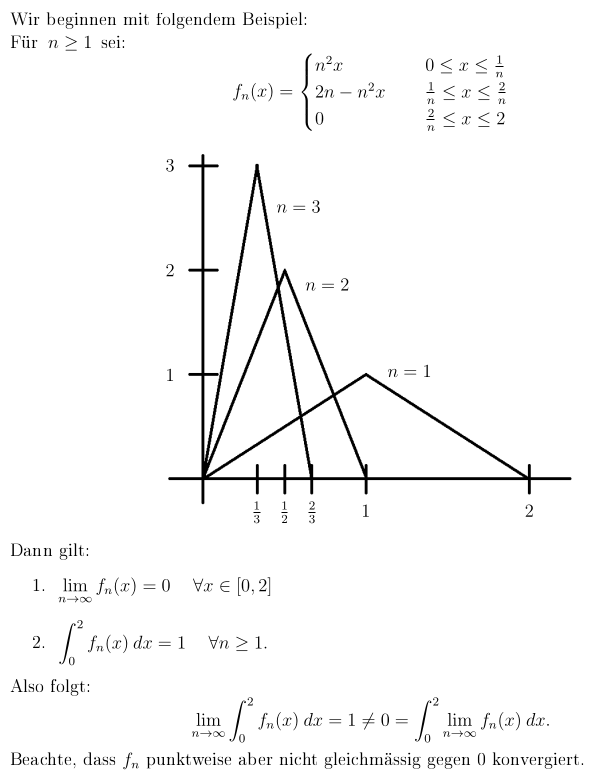
\includegraphics[scale=0.235]{Integration_konvergenterReihe.png} \newline
\Satz[5.34] Sei \(f_n : [a,b] \rightarrow \R \) eine Folge von beschränkten, integrierbaren Funktionen die gleichmässig gegen eine Funktion \(f:[a,b] \rightarrow \R \) konvergiert. Dann ist f beschränkt integrierbar und
\[ \lim\limits_{n \rightarrow \infty} \int_{a}^{b} f_n(x) \,dx = \int_{a}^{b} f(x) \,dx \]
\Korollar[5.35] Sei \(f_n : [a,b] \rightarrow \R\) eine Folge beschränkter integrierbarer Funktionen so dass
\[ \sum_{n=0}^\infty f_n\]
auf \([a.b]\) gleichmässig konvergiert. Dann gilt :
\[ \sum_{n=0}^\infty \int_{a}^{b} f_n(x) \,dx = \int_{a}^{b} \left( \sum_{n=0}^{\infty} f_n(x) \right) \,dx \]
\Korollar[5.36] Sei
\[ f(x) = \sum_{n=0}^{\infty} c_kx^k\]
eine Potenzreihe mit positivem Konvergenzradius \( \rho > 0\). Dann ist für jedes \( 0 \leq r < \rho\), f auf \([-r,r]\) integrierbar und es gilt \( \forall x \in ] -\rho, \rho[:\)
\[ \int_{0}^{x} f(t) dt = \sum_{n=0}^{\infty} \frac{c_n}{n+1} x^{n+1}\]
\sep
\subsection{Euler-McLaurin Summationsformel}
Diese Formel, ist ein sehr nützliches Instrument um Summen wie  \( 1 + \frac{1}{2} + \dots + \frac{1}{n}\)
oder \( \ln 1 + \ln 2 + \dots + \ln n = \ln n!\) abzuschätzen \newline
\Def[5.40] \( \forall k \geq 0 \) ist das k'te Bernoulli Polynom \(B_k(x) = k!P_k(x)\) Mit dieser Definition folgt: \(B_0(x) = 1, B_1(x) = x - \frac{1}{2}, B_2(x) = x^2 - x + \frac{1}{6}\)
\Def[5.41] Sei \(B_0 = 1\) für alle \( k \geq 2 \) definieren wir \(B_{k-1}\) rekursiv:
\[ \sum_{i=0}^{k-1} \binom{k}{i} B_i = 0\]
Also: \( B_0 = 1, B_0 + 2B_1 = 0, B_0 + 3B_1 + 3B_2 =0 \)
\Satz[5.42] \[ B_k(x) = \sum_{i=0}^{k} \binom{k}{i} B_ix^{k-i}\]
\Bem{5.43} Für \( k \geq 2\):

\begin{equation}
\begin{aligned}
B_{k}(1) &=\sum_{i=0}^{k}\left(\begin{array}{c}
k \\
i
\end{array}\right) B_{i}=\sum_{i=0}^{k-1}\left(\begin{array}{l}
k \\
i
\end{array}\right) B_{i}+B_{k} \\
&=B_{k} \quad(\text { nach } 5.41) \\
&=B_{k}(0) \quad(\text { nach Satz } 5.42)
\end{aligned}
\end{equation}

Zur Aussage der Summationsformel definieren wir für $k \geq 1$
$$
\widetilde{B}_{k}:[0, \infty[\longrightarrow \mathbb{R}
$$
als
$$
\widetilde{B}_{k}(x)=\left\{\begin{array}{ll}
B_{k}(x) & \text { für } \quad 0 \leq x<1 \\
B_{k}(x-n) & \text { für } n \leq x<n+1 \text { wobei } n \geq 1
\end{array}\right.
$$

\Satz[5.44] Sei \(f:[0,n] \rightarrow \R \) k-mal stetig differenzierbar, \(k \geq 1\). Dann gilt :
\begin{enumerate}
    \item [1] Für k = 1:
    \[ \sum_{i=1}^{n} f(i) = \int_{0}^{n} f(x) \,dx + \frac{1}{2} (f(n) - f(0))\]
    \[ + \int_{0}^{n} \tilde{B_1} (x) f'(x) \,dx \]
    \item [2] Für \( k \geq 2\):
    \[ \sum_{i=1}^{n}f(i) = \int_{0}^{n} f(x) \,dx + \frac{1}{2}(f(n) - f(0)) + \] 
    \[\sum_{J=2}^{k} \frac{(-1)^jB_j}{j!}(f^{(j-1)}(n) - f^{(j-1)}(0)) + \tilde{R_k}\]
    wobei
    \[ \tilde{R_k} = \frac{(-1)^{k-1}}{k!} \int_{0}^{n} \tilde{B_k}(x)f^{(k)}(x) \,dx \]
\end{enumerate}
\sep
\subsection{Stirling'sche Formel}
Die Stirling'sche Formel ist eine qualitative Aussage über das Verhalten der Fakultät
Nämlich:
\[ n! \approx \frac{\sqrt{2 \pi n} n^n}{e^n}\]
\Satz[5.47] \[n! = \frac{\sqrt{2 \pi n} n^n}{e^n} \cdot \exp(\frac{1}{12n}+ R_3(n))\]
wobei
\[ \abs{R_3(n)} \leq \frac{\sqrt{3}}{216 \cdot \frac{1}{n^2}} \quad \forall n \geq 1\]
\Lemma[5.48] \( \forall m \geq n + 1 \geq 1\):
\[ \abs{R_3(m,n)} \leq \frac{\sqrt{3}}{216}( \frac{1}{n^2} - \frac{1}{m^2})\]
\sep
\subsection{Uneigentliche Integrale}
Der Begriff des Riemann Integrals setzt voraus, dass \( [a,b]\) ein kompaktes Intervall und \(f: [a,b] \rightarrow \R \) beschränkt ist. Unter gewissen Vouraussetzungen kann man diese Einschränkung umgehen. \newline
\Def[5.49] Sei \(f:[a, \infty[ \rightarrow \R \) beschränkt und integrierbar auf \([a,b]\) für alle \( b > a\). Falls
\[ \lim\limits_{b \rightarrow \infty} \int_{a}^{b} f(x) \,dx \]
existiert, bezeichnen wir den Grenzwert mit
\[ \int_{a}^{\infty} f(x \,dx )\]
und sagen, dass f auf \([a, +\infty[ \) integrierbar ist.
\Bsp[5.50]
\begin{enumerate}
    \item \[\int_{0}^{\infty} e^{-x} d x=\lim _{b \rightarrow \infty} \int_{0}^{b} e^{-x} d x=\]
    \[\lim _{b \rightarrow \infty}\left(1-e^{-b}\right)=1\]
    \item $\int_{1}^{b} \frac{1}{x^{\alpha}} d x= \begin{cases}\ln b & \alpha=1 \\ \frac{b^{1-\alpha}-1}{1-\alpha} & \text { sonst. }\end{cases}$
\end{enumerate}
Somit: $\int_{1}^{\infty} \frac{1}{x^{\alpha}} d x=\left\{\begin{array}{cc}\text { divergiert, } & \alpha \leq 1 \\ \frac{1}{\alpha-1} & \alpha>1\end{array}\right.$
\Lemma[5.51] Sei \(f:[a, \infty [ \rightarrow \R \) beschränkt und integrierbar auf \([a,b] \quad \forall b > a\)
\begin{enumerate}
    \item [1] Falls \( \abs{f(x)} \leq g(x) \quad \forall x \geq a \) und \(g(x)\) ist auf \([a, \infty[ \) integrierbar, so ist f auf \([a, \infty[ \) integrierbar
    \item [2] Falls \( 0 \leq g(x) \leq f(x)\) und \(\int_{a}^{\infty} g(x)\) divergiert, so divergiert auch \( \int_{a}^{\infty} f(x) \,dx \)
\end{enumerate}
\Satz[5.53] (McLaurin 1742) Sei \(f : [1 , \infty[ \rightarrow [0, \infty[ \) monoton fallend. Die Reihe
\[ \sum_{n=1}^{\infty} f(n)\]
konvergiert genau dann, wenn
\[ \int_{1}^{\infty} f(x) \,dx \]
konvergiert \newline
Eine Situation die zu einem uneigentlichen Integral führt ist, falls
\[ f:]a,b[ \rightarrow \R\]
auf jedem Intervall \([a+\epsilon, b],\  \epsilon > 0 \) beschränkt und integrabel ist aber nicht notwendigerweise beschränkt auf \( ]a,b[\) \newline
\Def[5.56] In dieser Siutation ist \( f: ]a,b[ \rightarrow \R \) integrierbar falls
\[ \lim\limits_{\epsilon \rightarrow 0^{+}} \int_{a + \epsilon}^{b} f(x) \,dx \]
existiert; in diesem Fall wird der Grenzwert mit \(\int_{a}^{b} f(x) \,dx \) bezeichnet
\sep
\subsection{Die Gamma Funktion}
\Def[5.59] Für \(s > 0\) definieren wir
\[ \Gamma(s) := \int_{0}^{\infty} e^{-x}x^{s-1} \,dx\]
\Satz[5.60](Bohr-Mollerup)
\begin{enumerate}
    \item [1] Die Gamme Funktion erfüllt die Relationen
    \begin{enumerate}
        \item [(a)] \( \Gamma(1) = 1\)
        \item [(b)] \(\Gamma(s+1) = s\Gamma(s) \quad \forall s > 0 \)
        \item [(c)] \( \Gamma\) ist logarithmisch konvex, das heisst
        \[\Gamma( \lambda x + (1 - \lambda)y) \leq \Gamma(x)^{\lambda}\Gamma(y)^{1-\lambda}\]
        für alle \(x,y > 0\) und \(0 \leq \lambda \leq 1\)
    \end{enumerate}
    \item [2] Die Gamme Funktion ist die einzige Funktion \( 0, \infty[ \rightarrow ]0, \infty [\) die (a), (b) und (c) erfüllt. Darüber hinaus gilt:
    \[\Gamma(x) = \lim\limits_{n \rightarrow +\infty} \frac{n!n^x}{x(x+1) \dots (x+n)} \quad \forall x > 0\] 
\end{enumerate}
\Lemma[5.61] Sei \( \rho > 1\) und \(q > 1\) mit
\[ \frac{1}{p} + \frac{1}{q} = 1\]
Dann gilt \(\forall a,b \geq 0 \)
\[ a \cdot b \leq \frac{a^p}{p} + \frac{b^q}{q}\]
\Satz[5.62](Hölder Ungleichung). Seien \( \rho > 1\) und \( q > 1\) mit \( \frac{1}{p} + \frac{1}{q} = 1\). Für alle \(f,g : [a,b] \rightarrow \R \) stetig gilt:
\[ \int_{a}^{b} \abs{f(x)g(x)} \,dx \leq \abs{\abs{f}}_p \abs{\abs{g}}_q\]
\sep
\subsection{Das unbestimmte Integral}
\Def[Produktzerlegung]
Seien \( \alpha \pm i\beta_1. \dots , \alpha_l \pm i\beta_l\) sowie \( \gamma_1 \dots \gamma_k \) die paarweise verschiedene Wurzeln(Nullstellen) von Q,
wobei \( \alpha_j, \beta_j, \gamma_j\) reell und \(\beta_j \neq 0\). Dann lässt sich Q in ein Produkt zerlegen:
\[ Q(x) = \prod_{j=1}^l ((x- \alpha_j)^2 + \beta_j^2)^{m_j} \prod_{i=1}^k (x - \gamma_i)^{n_i}\]
\Satz[5.65] Seien P,Q Polynome mit grad(p) < grad(Q) und Q mit Produktzerlegung. Dann gibt es \( A_{ij}, B_{ij}, C_{ij}\) reelle Zahlen mit
\[ \frac{P(x)}{Q(x)} = \sum_{i=1}^l \sum_{j=1}^{m_i} \frac{(A_{ij} + B_{ij}x)}{((x - \alpha_i)^2 + \beta_i^2)^j} + \sum_{i=1}^k \sum_{j=1}^{n_i} \frac{C_{ij}}{(x - \gamma_i)^j}\]
\sep
\section{Tipps und Tricks}
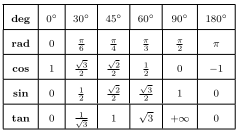
\includegraphics[scale=0.600]{RAD_values.png}
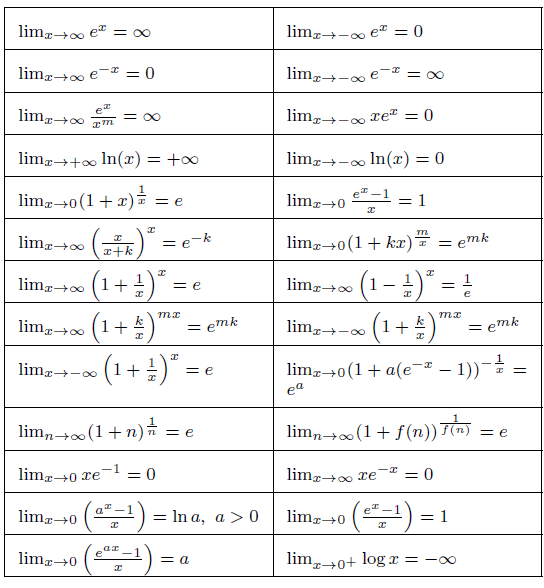
\includegraphics[scale=0.800]{RandomGrenzwerte.png}
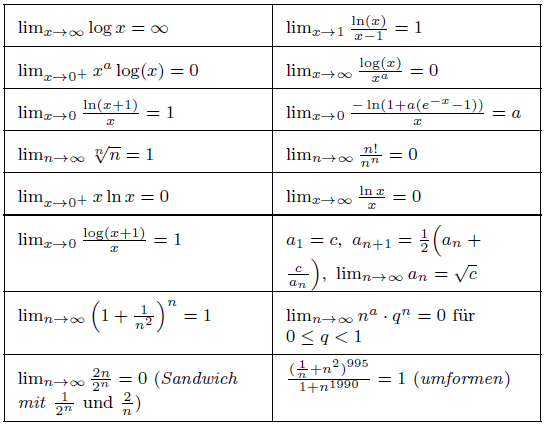
\includegraphics[scale=0.800]{randomGrenzwerte2.png}
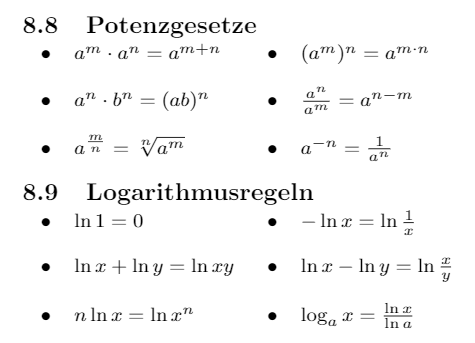
\includegraphics[scale=0.400]{logarithmus_Exponentengesetze.png}
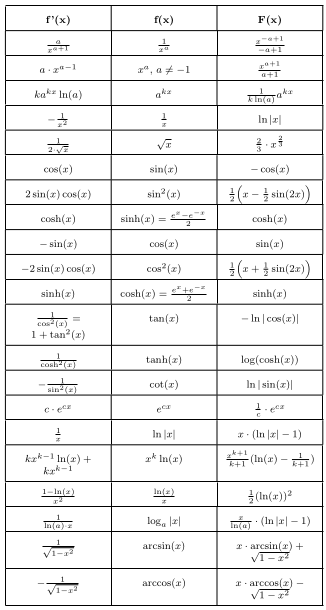
\includegraphics[scale=0.600]{randomIntegrale.png}
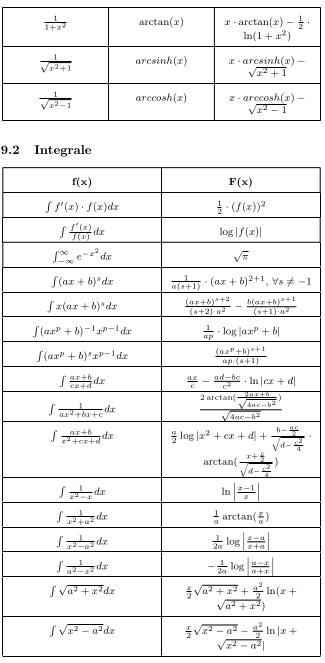
\includegraphics[scale=0.600]{randomIntegrale2.png}
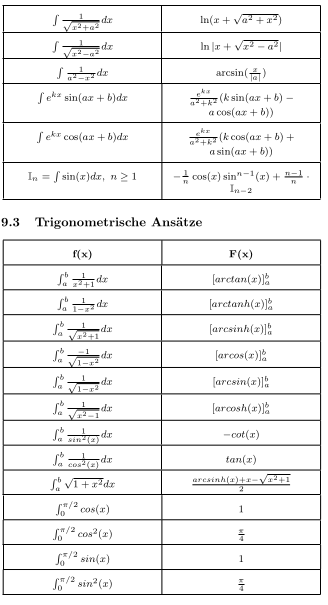
\includegraphics[scale=0.600]{randomIntegrale3.png}
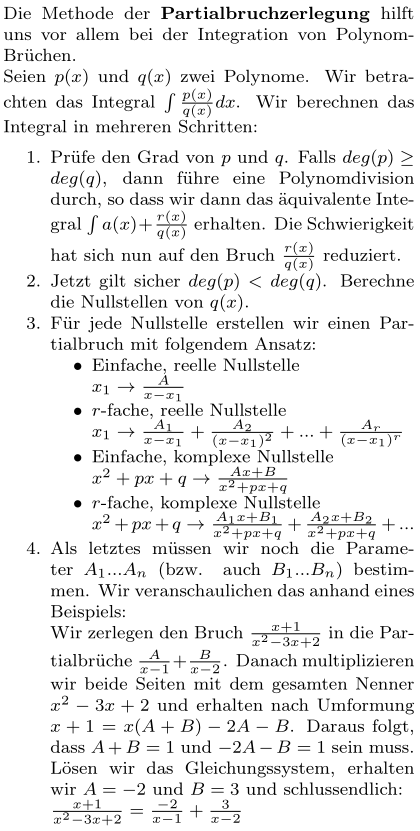
\includegraphics[scale=0.400]{Partialbruchzerlegung.png}